\documentclass{article}
\usepackage[pdftex]{graphicx}  
\begin{document}
\subsection{\bfseries Otvaranje računa}
\begin{figure}
\begin{center}
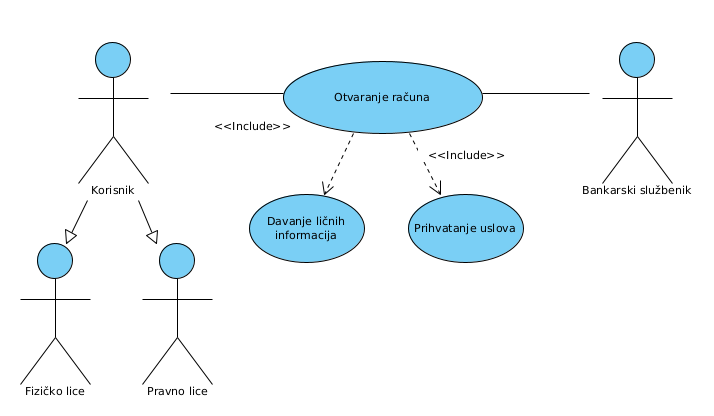
\includegraphics[scale=0.5]{./UseCases/Pictures/otvaranjeRacuna.png}
\end{center}
    \caption{Dijagram slučaja upotrebe otvaranja računa korisnika.}
\label{fig:Otvaranje računa}
\end{figure}


\subsubsection{ Otvaranje računa}

\begin{itemize}
    \item Kratak opis:
        \begin{itemize}
            \item Korisnik otvara račun u banci kako bi mogao da koristi pogodnosti koje ona nudi.
        \end{itemize}
    \item Učesnici:
        \begin{itemize}
            \item Zainteresovana osoba koja želi da ima račun u banci.
            \item Službeno lice koje je zaposleno u banci.
        \end{itemize}
    \item Preduslovi:
        \begin{itemize}
            \item Korisnik mora da bude punoletan.
            \item Korisnik mora da priloži tačne informacije.
            \item Korisnik mora da ima važeću ličnu kartu.
            \item Sistem mora biti u funkciji.
            \item Službeno lice mora biti autorizovano za korišćenje sistema.
        \end{itemize}
    \item Postuslovi:
        \begin{itemize}
            \item Korisnik je registrovan i ima otvoren račun u banci.
            \item Korisnik je ubačen u bazu podataka.
            \item Aktivirana je izrada korisnikove kartice.
        \end{itemize}
    \item Glavni tok:
        \begin{enumerate}
            \item Korisnik dolazi u filijalu i razgovara sa bankarskim službenikom.
            \item Bankarski službenik bira opciju za otvaranje novog računa.
            \item Sistem izbacuje formular.
            \item Službeno lice traži ličnu korisniku kartu.
            \item Korisnik prilaže ličnu kartu.
            \item Službeno lice popunjava u formularnu JMBG korisnika.
            \item Bankarski službenik ispituje korisnika o ostalim potrebnim informacijama.
            \item Korisnik daje tražene informacije.
            \begin{enumerate}
                \item Ukoliko je korisnik fizičko lice izvršava se podtok P1.
                \item Ukoliko je korisnik pravno lice izvršava se podtok P2.
            \end{enumerate}
            \item Službeno lice daje ugovor korisniku sa uslovima korišćenja računa u banci.
            \item Korisnik čita i prihvata uslove (potpisuje ugovor).
            \item Službenik unosi informacije u sistem i potvrdjuje unos.
            \item Sistem vrši validaciju podataka.
            \item Sistem čuva podatke.
            \item Bankarski službenik obaveštava korisnika da je račun aktiviran.
        \end{enumerate}
    \item Podtokovi:
        P1 Korisnik je fizičko lice:
        \begin{itemize}
            \item Ukoliko korisnik otvara račun kako bi primao platu mora dati podatke o firmi u kojoj radi.
        \end{itemize}   
        P2 Korisnik je pravno lice:
        \begin{itemize}
            \item Korisnik dostavlja rešenje o otvaranju firme (vlasnik firme, PIB, matični broj firme..) i karton deponovanih potpisa.
            \item Službeno lice izvlači rešenje o otvaranju firme iz APR-a.
            \item Službeno lice vrši proveru informacija tako što uporedjuje korisnikove i podatke iz APR-a.
            \item Službeno lice otvara novi formular i popunjava polja sa dostavljenim podacima.
            \item Službeno lice potvrdjuje unos u formularu.
            \item Služba za kontrolu dokumentacije pravnih lica vrši proveru unetih informacija.
            \item Unete informacije se čuvaju u sistemu.
        \end{itemize}    
    \item Alternativni tok:
        \begin{itemize}
            \item Prilikom 10. koraka glavnog toka korisnik odbija uslove otvaranja računa. Bankarski službenik poništava sve što je uneo u formular i svi podaci se brišu.
            \item Prilikom 12. koraka može doći do neuspešne validacije podataka, u tom slučaju sistem će izbaciti obaveštenje i biće onemogućeno čuvanje podataka dok se ne ispravi propust.
        \end{itemize}
    \item Dodatne informacije:
        \begin{itemize}
            \item Uslovi otvaranja računa u banci su regulisani zakonom. Nepoštovanje tih uslova može dovesti do sudskih postupaka.
        \end{itemize}
\end{itemize}

\end{document}
